\normaltrue
\correctiontrue

%\UPSTIidClasse{11} % 11 sup, 12 spé
%\newcommand{\UPSTIidClasse}{12}

\exer{Mouvement RT  $\star$ \label{C2:09:05}}
\setcounter{question}{0}\marginnote{\xpComp{DYN}{06}}%\UPSTIcompetence{C2-09}
\index{Compétence C2-09}\index{Compétence DYN-06}
\index{Principe fondamental de la dynamique}
\index{PFD}
\index{Mécanisme à 1 rotation et 1 translation}
\ifcorrection
\else
\marginnote{\textbf{Pas de corrigé pour cet exercice.}}
\fi

\ifprof
\else
Soit le mécanisme suivant. On a $\vect{AB}=\lambda(t)\vect{i_1}$. De plus :
\begin{itemize}
\item $G_1$ désigne le centre d'inertie de \textbf{1} et $\vect{AG_1}=L_1\vect{i_1}$, on note $m_1$ la masse de \textbf{1} et $\inertie{G_1}{1}=\matinertie{A_1}{B_1}{C_1}{0}{0}{0}{\bas{1}}$; 
\item $G_2=B$ désigne le centre d'inertie de \textbf{2}, on note $m_2$ la masse de \textbf{2} et $\inertie{G_2}{2}=\matinertie{A_2}{B_2}{C_2}{0}{0}{0}{\bas{2}}$.
\end{itemize}


Un moteur électrique positionné entre \textbf{0} et \textbf{1} permet d'actionner le solide \textbf{1}.
Un vérin électrique positionné entre \textbf{1} et \textbf{2} permet d'actionner le solide \textbf{2}

L'accélération de la pesanteur est donnée par $\vect{g}=-g\vect{j_0}$.

\begin{marginfigure}
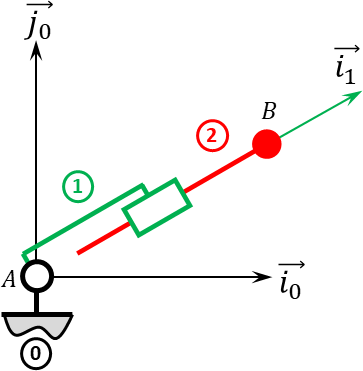
\includegraphics[width=\linewidth]{05_RT_01}
\end{marginfigure}
\fi

\question{Dans le but d'obtenir les lois de mouvement, appliquer le théorème de la résultante dynamique au solide \textbf{2} en projection sur $\vect{i_1}$.}
\ifprof

On isole le solide \textbf{2}.

On réalise le BAME : 
\begin{itemize}
\item liaison glissière : $\torseurstat{T}{1}{2}$ tel que $\vectf{1}{2}\cdot\vi{1} = 0$;
\item pesanteur sur 2 : $\torseurstat{T}{\text{pes}}{2} = \torseurl{-m_2 g \vj{0}}{\vect{0}}{B}$ avec $-m_2 g \vj{0} \cdot \vi{1} = -m_2 g\sin \theta$;
\item action du vérin $\torseurstat{T}{\text{Vérin}}{2} =  \torseurl{F_v \vi{1}}{\vect{0}}{A}$.
\end{itemize}

On applique le théorème de la résultante dynamique au solide 2 en projection sur $\vi{1}$ :
$\vectf{1}{2}\cdot\vi{1} + \left(-m_2 g \vj{0}\right) \cdot \vi{1} + F_v \vi{1}\cdot \vi{1} = \vectrd{2}{0}\cdot \vi{1}$.

Calcul de $\vectrd{2}{0}\cdot \vi{1}$ : 

$\vectrd{2}{0}\cdot \vi{1} = m_2\dderiv{\vect{AG_2}}{\rep{0}} \cdot \vi{1}$
$= m_2 \dderiv{\lambda(t) \vi{1} }{\rep{0}} \cdot \vi{1}$
$= m_2 \deriv{\lambdap(t) \vi{1} + \lambda(t) \thetap(t)\vj{1} }{\rep{0}} \cdot \vi{1}$

$= m_2 \left(\lambdapp(t) \vi{1} + \lambdap(t) \thetap(t)\vj{1} + \lambdap(t) \thetap(t)\vj{1}
+ \lambda(t) \thetapp(t)\vj{1}- \lambda(t) \thetap^2(t)\vi{1} \right) \cdot \vi{1}$
$= m_2 \left(\lambdapp(t)   - \lambda(t) \thetap^2(t) \right)$

Au final, l'application du TRD à 2 en projection sur $\vi{1}$ donne : 
$$ F_v-m_2 g\sin \theta = m_2 \left(\lambdapp(t)   - \lambda(t) \thetap^2(t) \right).$$
\else
\fi

\question{Dans le but d'obtenir les lois de mouvement, appliquer le théorème du moment dynamique à l'ensemble \textbf{1+2} au point $A$ en projection sur $\vect{k_0}$.}
\ifprof
On isole le solide \textbf{1+2}.

On réalise le BAME : 
\begin{itemize}
\item liaison pivot : $\torseurstat{T}{0}{1}$ tel que $\vectm{A}{0}{1}\cdot\vk{0} = 0$.
\item pesanteur sur 2 : $\torseurstat{T}{\text{pes}}{2} = \torseurl{-m_2 g \vj{0}}{\vect{0}}{B}$ avec 
$\vectm{A}{\text{pes}}{2} \cdot \vk{0} = \left(\vect{AB}\wedge -m_2 g \vj{0} \right)\cdot \vk{0}$
$= \left(\lambda(t) \vi{1} \wedge -m_2 g \vj{0} \right)\cdot \vk{0}$
$= -m_2 g\lambda(t)\cos\theta(t) $;

\item pesanteur sur 1 : $\torseurstat{T}{\text{pes}}{1} = \torseurl{-m_1 g \vj{0}}{\vect{0}}{G_1}$ avec 
$\vectm{A}{\text{pes}}{1} \cdot \vk{0} = \left(\vect{AG_1}\wedge -m_1 g \vj{0} \right)\cdot \vk{0}$
$= \left(L_1 \vi{1}\wedge -m_1 g \vj{0} \right)\cdot \vk{0}$
$= -m_1 gL_1\cos\theta(t) $;

\item action du moteur $\torseurstat{T}{\text{Moteur}}{1} =  \torseurl{\vect{0}}{C_m \vk{0}}{A}$.
\end{itemize}

\vspace{.5cm}

On applique le théorème du moment dynamique au solide 1+2 en projection sur $\vk{0}$ :
$
\vectm{A}{0}{1}\cdot\vk{0} 
+ \vectm{A}{\text{pes}}{2} \cdot \vk{0}
+ \vectm{A}{\text{pes}}{1} \cdot \vk{0} + C_m \vk{0}
= \vectmd{A}{1+2}{0} \cdot \vk{0}$.

\vspace{.5cm}

Calcul de $\vectmd{A}{1+2}{0} \cdot \vk{0} = \vectmd{A}{1}{0} \cdot \vk{0} + \vectmd{A}{2}{0} \cdot \vk{0} $.

\vspace{.5cm}

Calcul de $\vectmd{A}{1}{0} \cdot \vk{0}$ : 

$\vectmd{A}{1}{0} \cdot \vk{0}$ 
$=\left(\vectmd{G_1}{1}{0} + \vect{AG_1} \wedge \vectrd{1}{0} \right)\cdot \vk{0}$
$=\left( \deriv{\vectmc{G_1}{1}{0}}{0} + m_1 \vect{AG_1} \wedge \dderiv{\vect{AG_1}}{0} \right)\cdot \vk{0}$

$=\left( \deriv{\vectmc{G_1}{1}{0}}{0}\cdot \vk{0} + \left(m_1 \vect{AG_1} \wedge \dderiv{\vect{AG_1}}{0}\right)\cdot \vk{0} \right)$

$=\left( \deriv{\vectmc{G_1}{1}{0}\cdot \vk{0}}{0} + \left(m_1 L_1 \vi{1} \wedge \left( L_1 \thetapp(t)\vj{1}-L_1  \thetap^2(t)\vi{1}\right)\right)\cdot \vk{0} \right)$ car $\deriv{\vk{0}}{0}=\vect{0}$.


$= C_1 \thetapp(t) + m_1 L_1^2 \thetapp(t)$ 

\vspace{.5cm}

Calcul de $\vectmd{A}{2}{0} \cdot \vk{0}$

$\vectmd{A}{2}{0} \cdot \vk{0}$ 
$=\left(\vectmd{G_2}{2}{0} + \vect{AG_2} \wedge \vectrd{2}{0} \right)\cdot \vk{0}$
$=\left( \deriv{\vectmc{B}{2}{0}}{0} + m_2 \vect{AB} \wedge \dderiv{AB}{0} \right)\cdot \vk{0}$

$=\left( \deriv{\vectmc{B}{2}{0}}{0}\cdot \vk{0} + \left(m_2 \vect{AB} \wedge \dderiv{\vAB}{0}\right)\cdot \vk{0} \right)$

$=\left( \deriv{\vectmc{B}{2}{0}\cdot \vk{0}}{0} + \left(m_2 \lambda(t) \vi{1} \wedge \left( \lambdapp(t) \vi{1} + \lambdap(t) \thetap(t)\vj{1} + \lambdap(t) \thetap(t)\vj{1}
+ \lambda(t) \thetapp(t)\vj{1}- \lambda(t) \thetap^2(t)\vi{1}\right)\right)\cdot \vk{0} \right)$ car $\deriv{\vk{0}}{0}=\vect{0}$.

$= C_2 \thetapp(t) + m_2 \lambda(t)  \left(  \lambdap(t) \thetap(t) + \lambdap(t) \thetap(t) + \lambda(t) \thetapp(t)\right)$.

\vspace{.5cm}

On a donc (j'espère ...) :
$$ C_m -m_1 gL_1\cos\theta(t)-m_2 g\lambda(t)\cos\theta(t) =
C_1 \thetapp(t) + m_1 L_1^2 \thetapp(t)
+C_2 \thetapp(t) + m_2 \lambda(t)  \left(  2\lambdap(t) \thetap(t)  + \lambda(t) \thetapp(t)\right).
$$

$$ C_m - \left(m_1 L_1+m_2 \lambda(t)\right) g \cos\theta(t) =
C_1 \thetapp(t) + m_1 L_1^2 \thetapp(t)
+C_2 \thetapp(t) +    2m_2 \lambda(t)\lambdap(t) \thetap(t)  + m_2 \lambda^2(t) \thetapp(t).
$$

\else
\fi


\ifprof
\else
\footnotesize
\begin{marginfigure}
\begin{tabular}{|p{.9\linewidth}|}
\hline
Eléments de correction : 
\begin{enumerate}
 \item $ F_v-m_2 g\sin \theta = m_2 \left(\lambdapp(t)   - \lambda(t) \thetap^2(t) \right)$.
\item  $C_m - \left(m_1 L_1+m_2 \lambda(t)\right) g \cos\theta(t) =
C_1 \thetapp(t) + m_1 L_1^2 \thetapp(t)
+C_2 \thetapp(t) +    2m_2 \lambda(t)\lambdap(t) \thetap(t)  + m_2 \lambda^2(t) \thetapp(t)
$. 
\end{enumerate} \\
\hline
\end{tabular}
\end{marginfigure}
\normalsize


\marginnote{Corrigé voir \ref{C2:09:05}.}

\fi